\documentclass[10pt]{beamer}
\usetheme{jambro}

\title[]{Métodos Quantitativos em Economia I - Apresentação}
\author[]{Paulo Victor da Fonseca}
\date{01 de março de 2023}

\hypersetup{
    colorlinks = true,
    urlcolor = teal,
    linkcolor = white    
}
\usepackage[portuguese]{babel}
\usepackage{subfig}
\usepackage{emoji}

\newtheorem{obj}{Objetivo}
\newtheorem{ementa}{Ementa}

\begin{document}

\begin{frame}[plain]
    \titlepage{
        \begin{center}
            \begin{minipage}{0.8\textwidth}
                \centering
            \end{minipage}
        \end{center}}
\end{frame}

\section{Docente}
\begin{frame}{Docente}
    \begin{tabular}{cl}
        \begin{tabular}{c}
            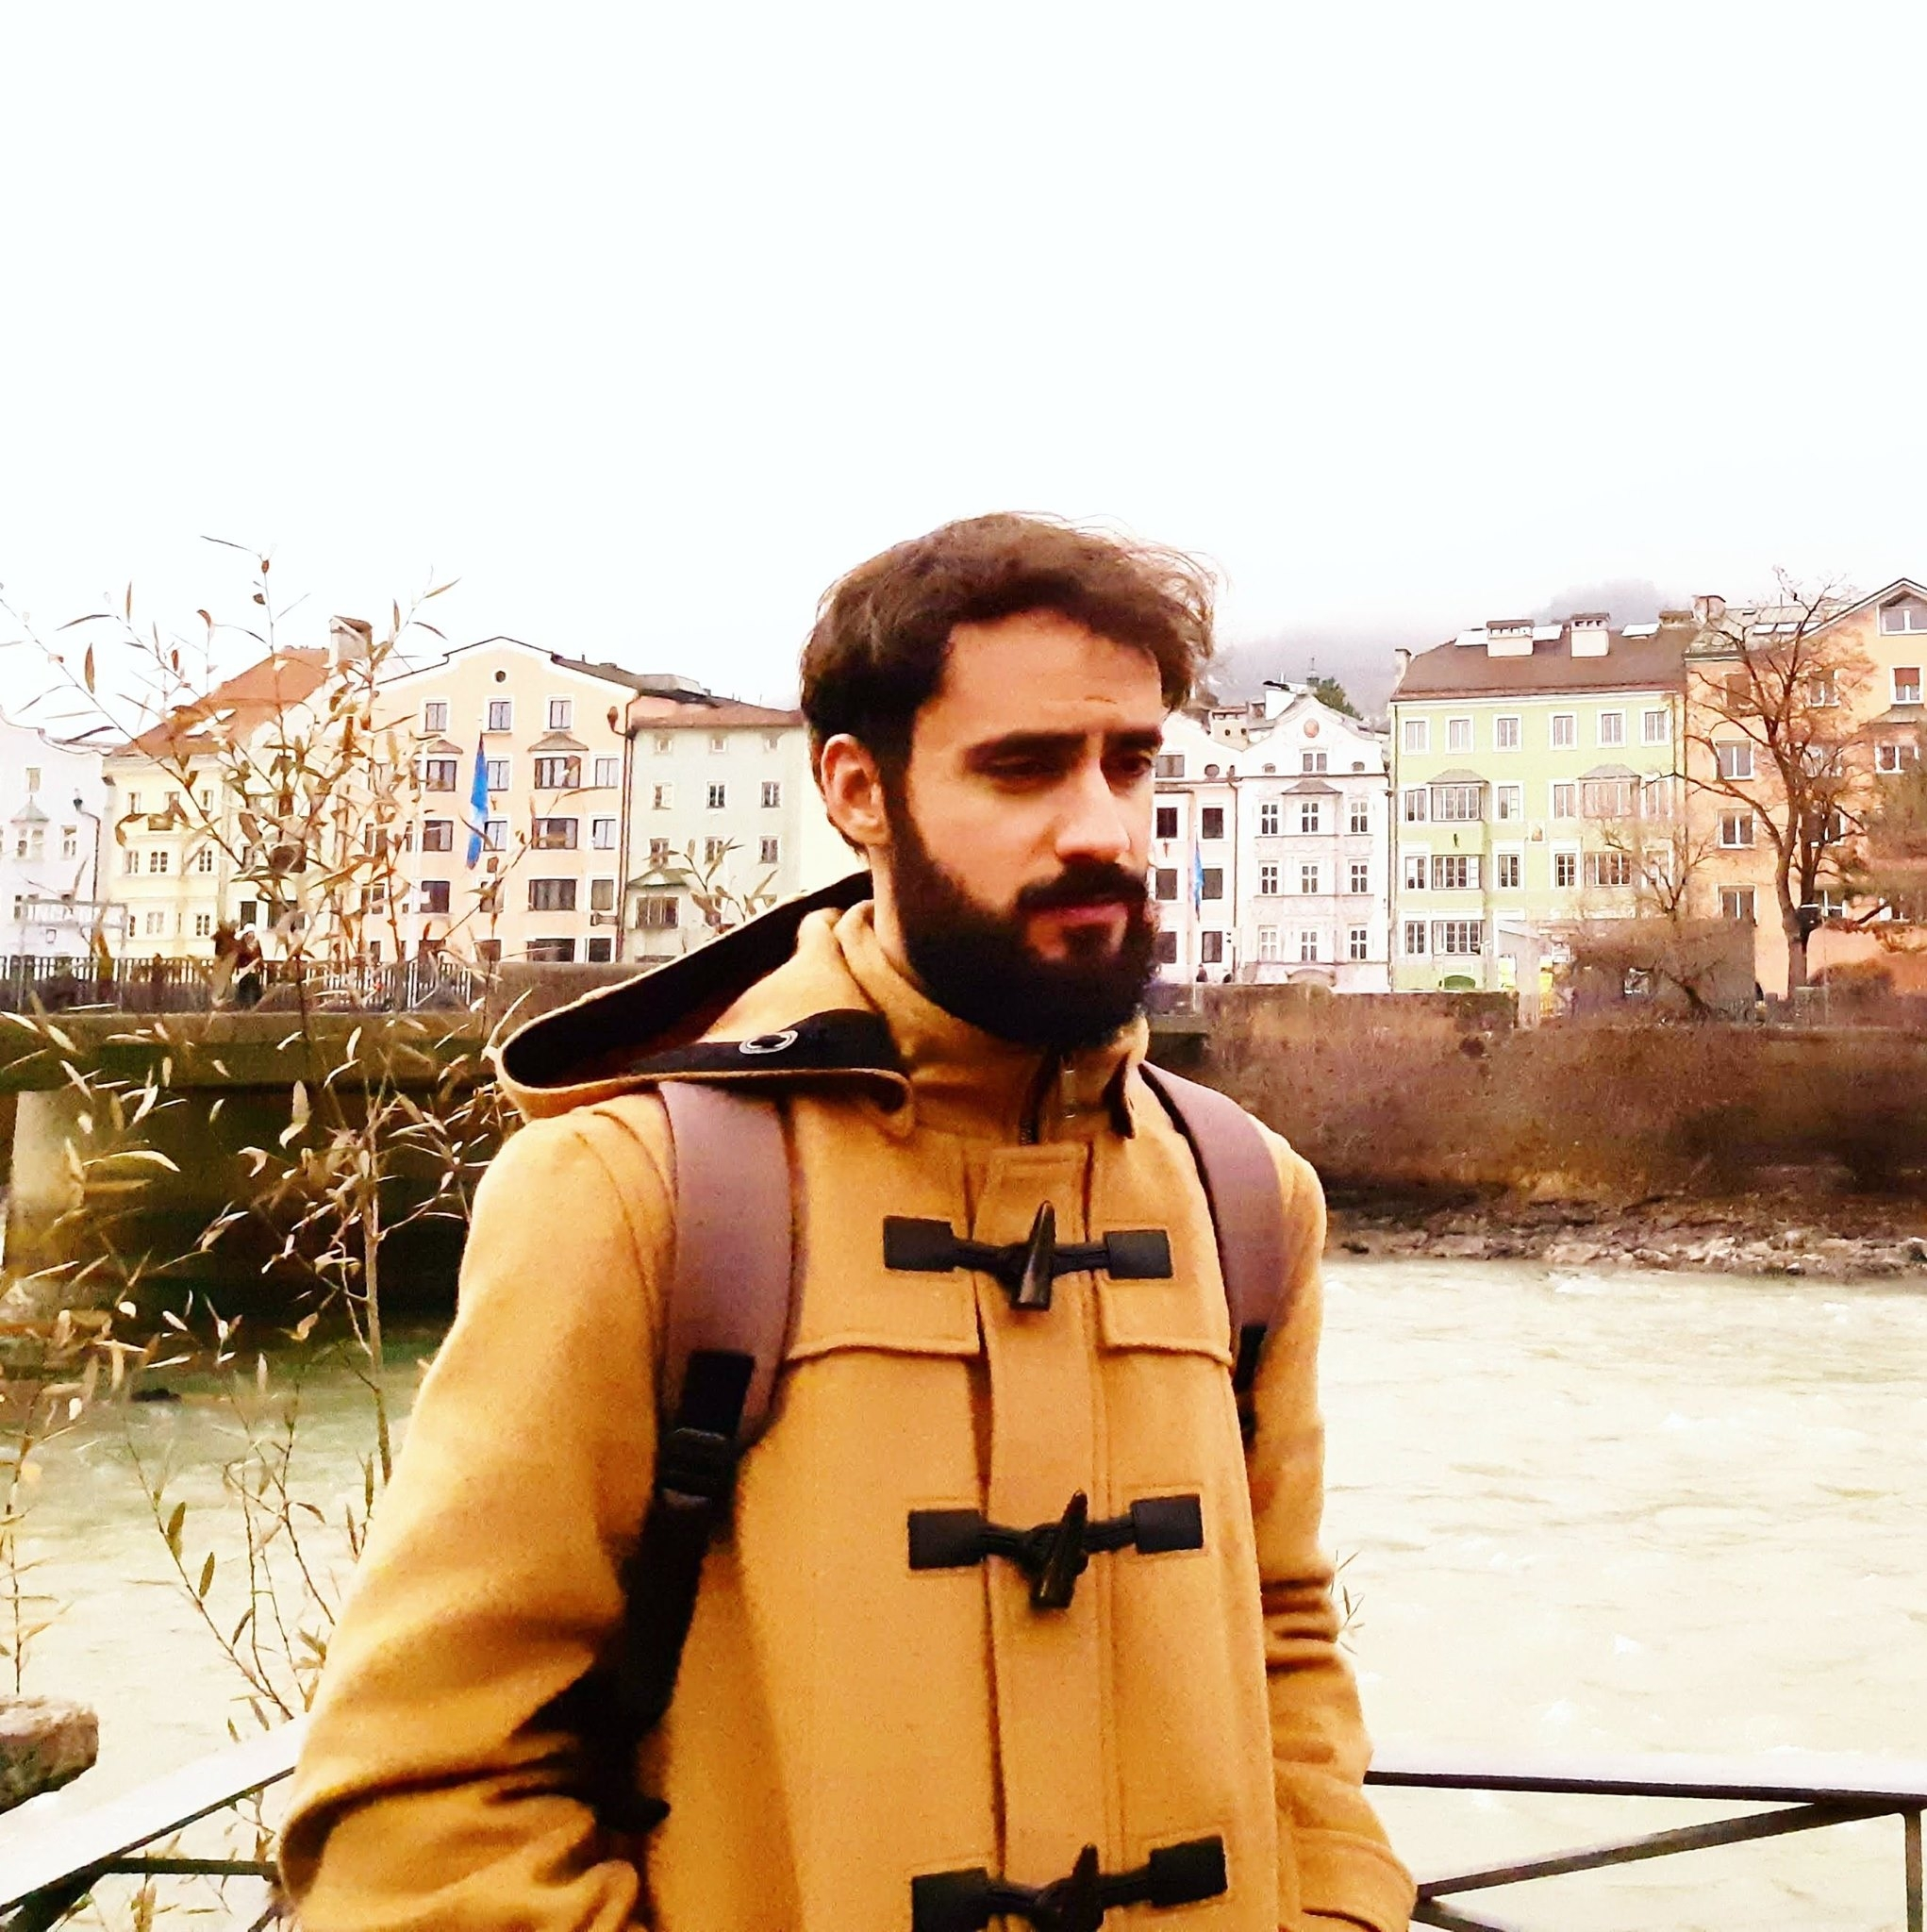
\includegraphics[width=3.5cm]{./figures/Paulo}
        \end{tabular}
         & \begin{tabular}{l}
               \parbox{0.6\linewidth}{%  change the parbox width as appropiate
                   \begin{itemize}
                    \item \textbf{Nome:} Paulo Victor da Fonseca\medskip
                    \item \textbf{Formação:} Doutorado em Economia - UFSC\medskip
                    \item \textbf{Áreas de pesquisa:} Macroeconomia. Políticas monetária e fiscal. Modelos DSGE. Modelos novo-Keynesianos com agentes heterogêneos. Modelos baseados em agentes.\medskip
                    \item \textbf{Website:} \href{https://pvfonseca.github.io}{pvfonseca.github.io}\medskip
                    \item \textbf{Contato:} \href{mailto:paulo.fonseca@udesc.br}{paulo.fonseca@udesc.br}
                \end{itemize}
               }
           \end{tabular} \\
    \end{tabular}
\end{frame}

\section{Motivação}
\begin{frame}{Métodos Quantitativos em Economia I}
    \begin{center}
        \begin{minipage}{0.8\textwidth}
            \begin{figure}
                \href{https://pvfonseca.github.io/html/mqe_aula01.html}{\includegraphics[width=\textwidth]{./figures/apresentacao.png}}
            \end{figure}
        \end{minipage}
    \end{center}
\end{frame}

\section{Ementa}
\begin{frame}{Métodos Quantitativos em Economia I: Ementa}
    \begin{center}
        \begin{minipage}{.9\textwidth}
            \NB{\hlight{Otimiza\c{c}\~{a}o irrestrita:} Condições de 1ª e 2ª ordens para máximos e mínimos irrestritos. Aplicações econômicas de otimização irrestrita.\medskip \\
            \hlight{Otimiza\c{c}\~{a}o com restri\c{c}\~{o}es:} Condições de 1ª ordem para otimização condicionada com restrições de igualdade e desigualdade.  Método dos multiplicadores de Lagrange e de Kuhn Tucker. Condições de 2ª ordem para otimização condicionada com restrições de igualdade e desigualdade.  Interpretação dos multiplicadores em problemas de otimização.  Teorema do envelope. \medskip \\
            \hlight{Homogeneidade, homoteticidade, concavidade, quase-concavidade:} Funções homogêneas, homotéticas, côncavas e quase côncavas. \medskip \\
            \hlight{Aplica\c{c}\~{o}es econ\^{o}micas:} Aplicações econômicas dos problemas de otimização relacionados à maximização de utilidade e demanda maximização de lucros, custos, ótimo de Pareto e teoremas fundamentais de bem-estar. \medskip \\
            \hlight{Programa\c{c}\~{a}o linear:} Programação linear.
            }
        \end{minipage}
    \end{center}

\end{frame}

\section{Objetivo}
\begin{frame}{Métodos Quantitativos em Economia I: objetivo}
    \begin{center}
        \begin{minipage}{.9\textwidth}
            \NB{O objetivo da disciplina é apresentar aos alunos as principais técnicas de otimização estática, bem como suas principais aplicações em Economia. \\
                Ao final do curso espera-se que o aluno seja capaz de utilizar o ferramental desenvolvido na disciplina em aplicações à Teoria Econômica (microeconomia, macroeconomia e disciplinas correlatas).}
        \end{minipage}
    \end{center}

    O curso será dividido em seis blocos:\medskip
    \begin{enumerate}
        \item Introdução e revisão de conceitos básicos\medskip

        \item Otimização estática sem restrições\medskip

        \item Otimização estática com restrições\medskip

        \item Funções homogêneas e funções homotéticas\medskip

        \item Concavidade e quase-concavidade\medskip

        \item Programação linear
    \end{enumerate}
\end{frame}

\section{Formato das aulas e avaliações}
\begin{frame}{Formato das aulas e sistema de avaliação}
    \begin{itemize}
        \item A disciplina apoia-se, fundamentalmente, em livros-texto e notas de aula e será ministrada por meio de aulas expositivas.\bigskip

        \item As aulas acontecerão às:
              \begin{itemize}
                  \item Quartas-feiras das 10:15 às 11:55
                  \item Sextas-feiras das 10:15 às 11:55\bigskip
              \end{itemize}

        \item A avaliação será realizada a partir dos procedimentos abaixo:
              \begin{itemize}
                  \item Atividade avaliativa I (PI): 30\%
                  \item Atividade avaliativa II (PII): 30\%
                  \item Atividade avaliativa III (PIII): 20\%
                  \item Trabalhos adicionais: 20\%\bigskip
              \end{itemize}

        \item Página da disciplina no GitHub: \href{github.com/pvfonseca/MetodosQuantitativos}{https://github.com/pvfonseca/MetodosQuantitativos}
    \end{itemize}
\end{frame}

\begin{frame}{Formato das aulas e sistema de avaliação}
    \begin{itemize}
        \item Os alunos devem ter em mente que o aprendizado e o acompanhamento do curso dependem essencialmente de seu próprio esforço.\bigskip

        \item Os tópicos do programa serão apresentados em aulas expositivas, destinadas à apresentação de conceitos, modelos e suas aplicações.\bigskip

        \item[\emoji{warning}] \hlight{Embora importantes, as aulas n\~{a}o podem jamais ser vistas como substitutas da leitura regular e cuidadosa dos textos indicados e da resolu\c{c}\~{a}o dos exerc\'{i}cios propostos.}
    \end{itemize}

\end{frame}
\section{Bibliografia}

\begin{frame}{Bibliografia}
    \begin{figure}
        \centering
        \subfloat[Chiang e Wainwright (2006)\label{fig1a}]{\includegraphics[width=0.2\textwidth]{./figures/chiang}} \quad
        \subfloat[Simon e Blume (2004)\label{fig1b}]{\includegraphics[width=0.2\textwidth]{./figures/simon}} \quad
        \subfloat[Hoy et al. (2022)\label{fig1c}]{\includegraphics[width=0.25\textwidth]{./figures/hoy}} \quad
        \subfloat[Nicholson e Snyder (2019)\label{fig1d}]{\includegraphics[width=0.2\textwidth]{./figures/nicholson}}
        \caption{Bibliografia do curso}
        \label{fig1}
    \end{figure}
\end{frame}

\begin{frame}{Bibliografia}
    \begin{figure}
        \centering
        \subfloat[Dixit (1990)\label{fig3a}]{\includegraphics[width=0.25\textwidth]{./figures/dixit}} \quad
        \subfloat[Fuente (2000)\label{fig3b}]{\includegraphics[width=0.25\textwidth]{./figures/fuente}} \quad
        \subfloat[Sydsaeter et al. (2016)\label{fig3c}]{\includegraphics[width=0.25\textwidth]{./figures/carvajal}}
        \caption{Bibliografia do curso}
        \label{fig3}
    \end{figure}
\end{frame}

\begin{frame}{Bibliografia}
    \begin{figure}
        \centering
        \subfloat[Silberberg e Suen (2001)\label{fig2b}]{\includegraphics[width=0.25\textwidth]{./figures/silberberg}} \quad
        \subfloat[Stewart (2017)\label{fig2c}]{\includegraphics[width=0.25\textwidth]{./figures/stewart1}} \quad
        \subfloat[Stewart (2017)\label{fig2d}]{\includegraphics[width=0.25\textwidth]{./figures/stewart2}}
        \caption{Bibliografia do curso}
        \label{fig2}
    \end{figure}
\end{frame}

\begin{frame}{Bibliografia}
    \begin{itemize}
        \item CHIANG, A.C.; WAINWRIGHT, K. \emph{Matemática para economistas}. Rio de Janeiro: Elsevier, 2006.
        \item DIXIT, A. \emph{Optimization in Economic Theory}. 2.ed., Oxford University Press, 1990.
        \item HOY, M.; LIVERNOIS, J.; McKENNA, C.; REES, R.; STENGOS, T. \emph{Mathematics for Economics}. 2.ed., Massachusetts: MIT Press, 2001.
        \item FUENTE, A. \emph{Mathematical methods and models for economists}. Cambridge, UK. New York, NY: Cambridge University Press, 2000.
        \item NICHOLSON, W.; SNYDER C. \emph{Teoria microeconômica: Princípios básicos e aplicações}. Cengage Learning Brasil, 2019. Disponível em: \href{https://app.minhabiblioteca.com.br/books/9788522127030/}{app.minhabiblioteca.com.br/books/9788522127030}
        \item SILBERBERG, E.; SUEN, W. \emph{The structure of economics: a mathematical analysis}. 3rd.ed. Singapore: McGraw-Hill Higher Education, 2001.
        \item SIMON, C.P.; BLUME, L. \emph{Matemática para economistas}. Porto Alegre: Bookman, 2004.
        \item STEWART, J. \emph{Cálculo – Volume 1}. 8.ed. Cengage Learning Brasil, 2017. Disponível em: \href{https://app.minhabiblioteca.com.br/books/9788522126859/}{app.minhabiblioteca.com.br/books/9788522126859}
        \item STEWART, J. \emph{Cálculo – Volume 2}. 8.ed. Cengage Learning Brasil, 2017. Disponível em: \href{https://app.minhabiblioteca.com.br/books/9788522126866/}{app.minhabiblioteca.com.br/books/9788522126866}
        \item SYDSÆTER, K.; HAMMOND, P.J.; STRØM, A.; CARVAJAL, A. \emph{Essential mathematics for economic analysis}. 5th.ed. Harlow, UK: Pearson Education Limited, 2016.
    \end{itemize}
\end{frame}
\end{document}